Based on a principal component analysis of the data (excluding the first columns including only identifier information like state names) there appear to be some potential problems with outliers. In all PCA illustrations, the colors represent amount of auto theft.

\begin{figure}[H]
\centering
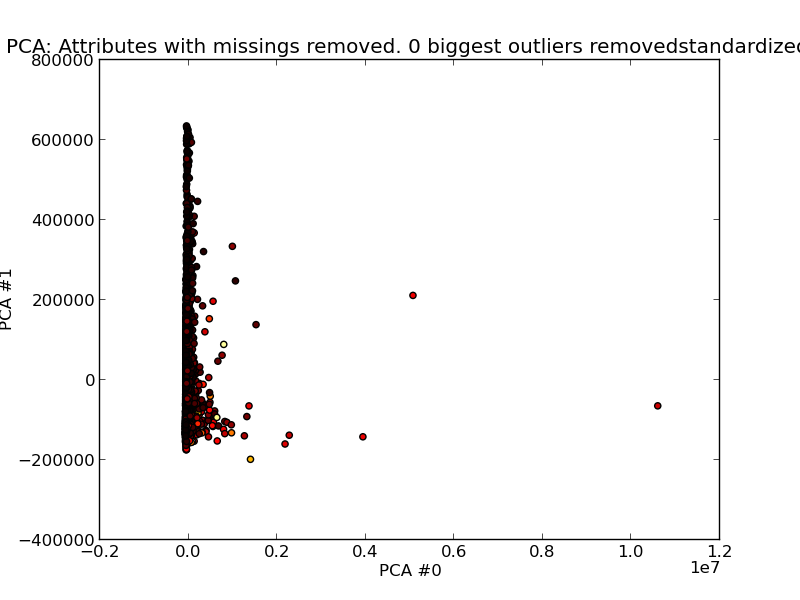
\includegraphics[width=0.9\textwidth]{pca/attr-with-missings-removed_0-biggest-outliers-removed_standrd_}
\label{fig:prenorm_attrrem_0out}
\caption{PCA, where attributes with missing values have been removed removed.}
\end{figure}

We are not yet sure how best to deal with these, but in order to explore our data we also performed principal componenet analysis on our data set with some of the biggest outliers removed.

\begin{figure}[H]
\centering
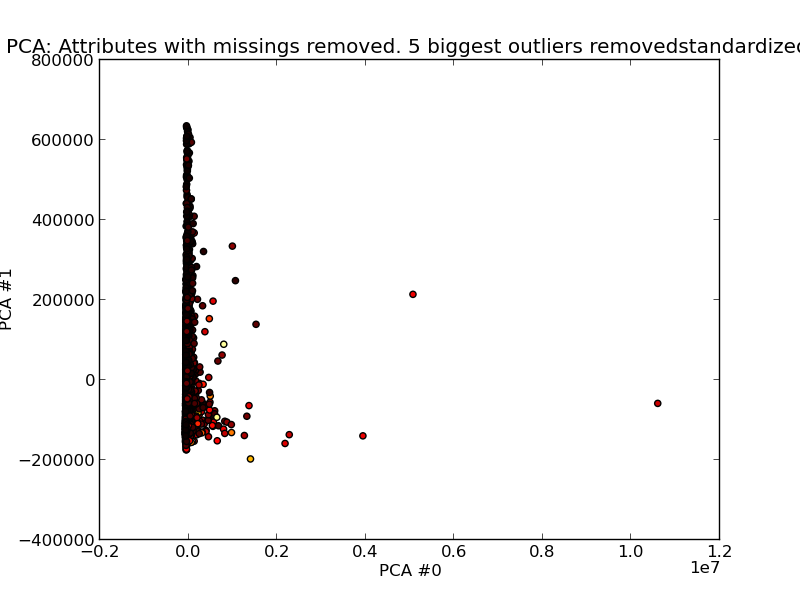
\includegraphics[width=0.9\textwidth]{pca/attr-with-missings-removed_5-biggest-outliers-removed_standrd_}
\label{fig:prenorm_attrrem_0out}
\caption{PCA, where attributes with missing values have been removed removed. Also the 5 biggest outliers from before have been removed prior to PCA.}
\end{figure}

The above pictures illustrate our results, when we dealt with missing values by removing the corresponding attribute completely. We also performed PCA after removing data objects with missing values instead, see below


\begin{figure}[H]
\centering
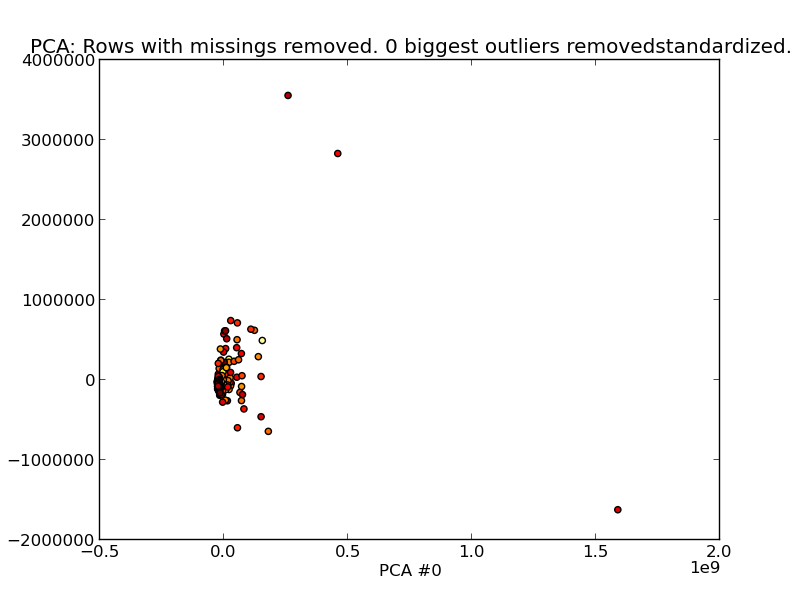
\includegraphics[width=0.9\textwidth]{pca/rows-with-missings-removed_0-biggest-outliers-removed_standrd_}
\label{fig:prenorm_attrrem_0out}
\caption{PCA, where data objects with missing values have been removed removed.}
\end{figure}
\begin{figure}[H]
\centering
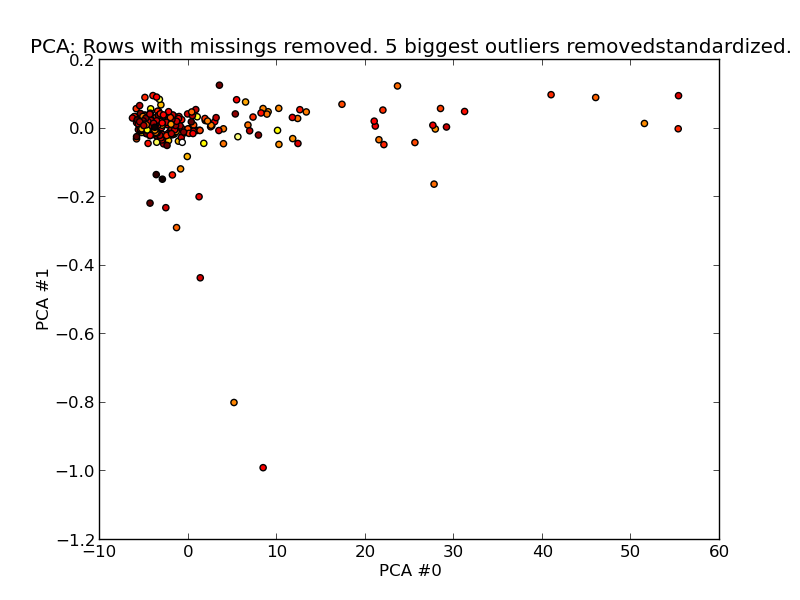
\includegraphics[width=0.9\textwidth]{pca/rows-with-missings-removed_5-biggest-outliers-removed_standrd_}
\label{fig:prenorm_attrrem_0out}
\caption{PCA, where data objects with missing values have been removed removed. Also the 5 biggest outliers from before have been removed prior to PCA.}
\end{figure}

We also did PCA where we simply put the means along attributes instead of missing values, producing the following principal components.

\begin{figure}[H]
\centering
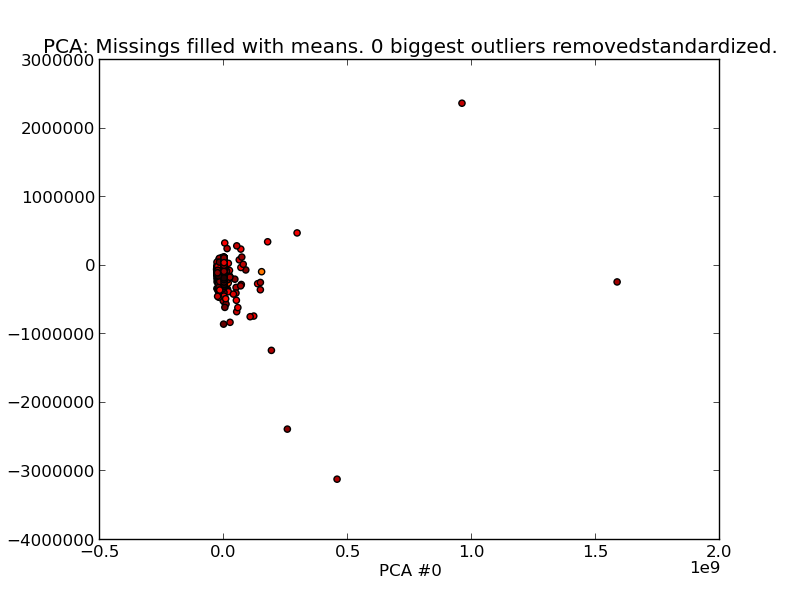
\includegraphics[width=0.9\textwidth]{pca/missings-filled-w-means_0-biggest-outliers-removed_standrd_}
\label{fig:prenorm_attrrem_0out}
\caption{PCA, where missing values have been replaced with means.}
\end{figure}
\begin{figure}[H]
\centering
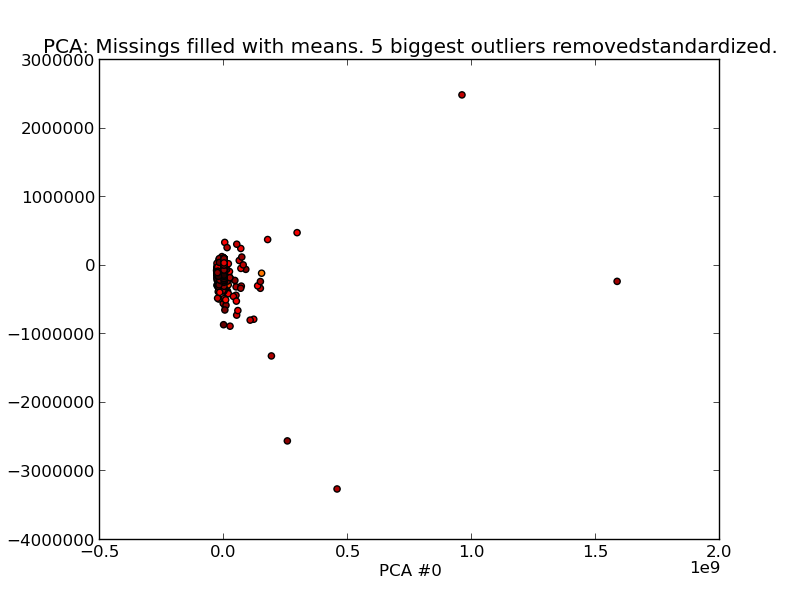
\includegraphics[width=0.9\textwidth]{pca/missings-filled-w-means_5-biggest-outliers-removed_standrd_}
\label{fig:prenorm_attrrem_0out}
\caption{PCA, where missing values have been replaced with means. Also the 5 biggest outliers from before have been removed prior to PCA.}
\end{figure}

Investigating the work others have performed on the data, leads us to believe that considerably better preprocessing can be done to the data. As an example, we have performed principal component analysis also on the normalized data set produced by [WHO].

\begin{figure}[H]
\centering
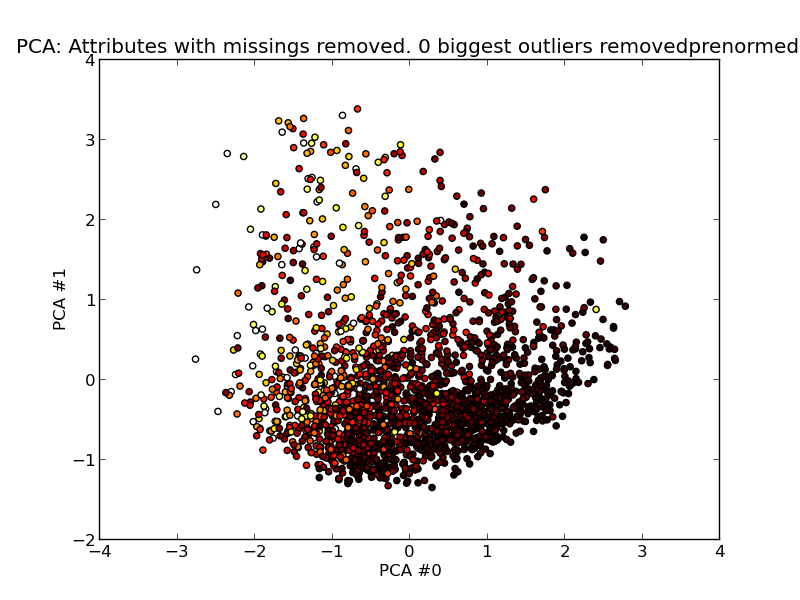
\includegraphics[width=0.9\textwidth]{pca/attr-with-missings-removed_0-biggest-outliers-removed_prenormed_}
\label{fig:prenorm_attrrem_0out}
\caption{Using normalized data from other source, attributes with missing values are removed.}
\end{figure}

The above data also appears to be normally distributed, in contrast to our own PCA. The first principal component also seems to capture quite well the amount of auto theft.

\begin{figure}[H]
\centering
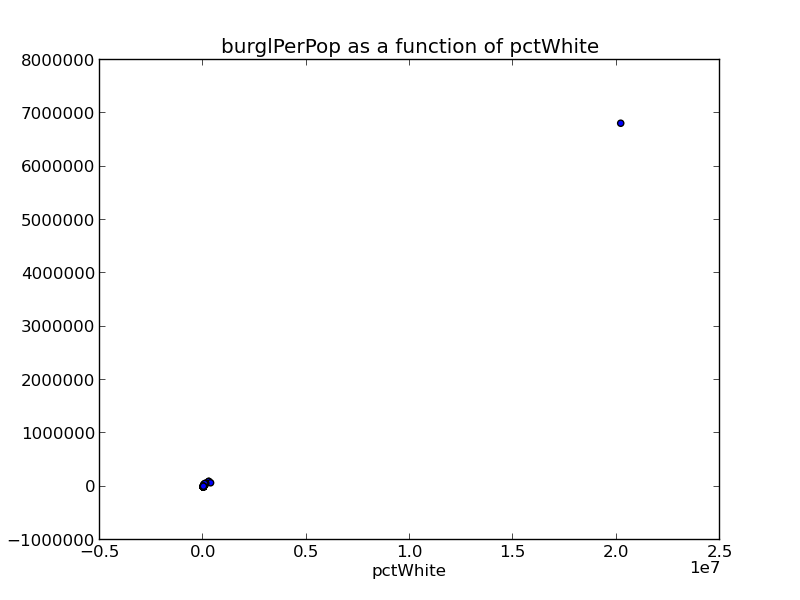
\includegraphics[width=0.9\textwidth]{correlations/burglPerPop-as-func-of-pctWhite.png}
\label{fig:prenorm_attrrem_0out}
\caption{Burgleries per population (1K people) as function of percentage of white population.}
\end{figure}

Many of our attributes have little correlation, as seen above, which is why regression is an obvious machine learning task. Looking at the normalized data by [WHO], furthermore leads us to believe that the task is feasable.

There are, however, some obvious attributes with high correlation, like population and auto theft, as seen below.

\begin{figure}[H]
\centering
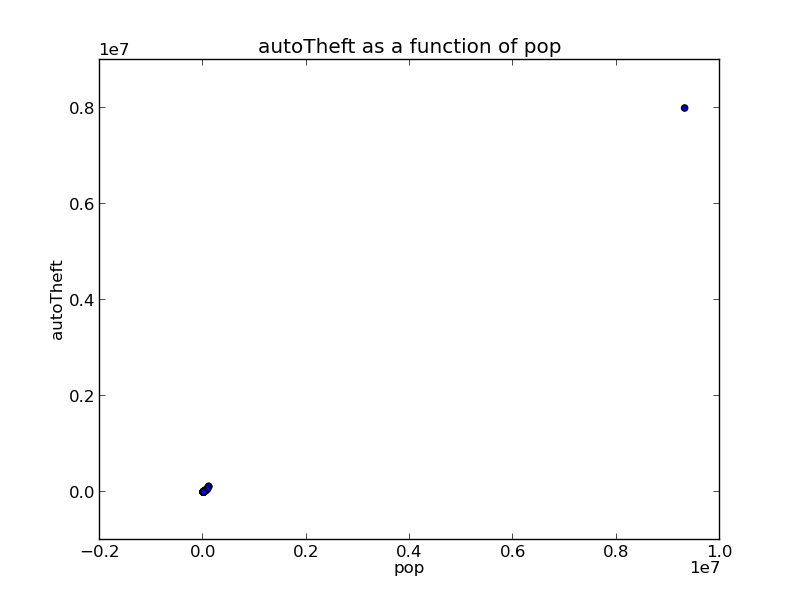
\includegraphics[width=0.9\textwidth]{correlations/autoTheft-as-func-of-pop}
\label{fig:prenorm_attrrem_0out}
\caption{Auto theft as function of population.}
\end{figure}

We realize now, that a possible problem with our principal component analysis is that we kept all of the violent crime attributes, which have very high correlation.
